% A TikZ scale on the picture scales the whole axis image, text and line widths
% included (behaviour Z1; real documents: tikzpicture[scale=0.7] around an axis).
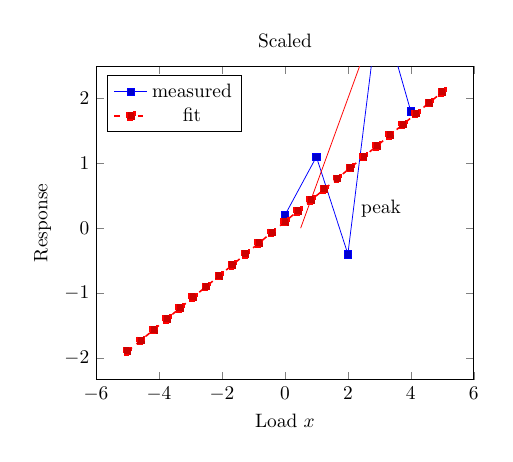
\begin{tikzpicture}[scale=0.7]
\begin{axis}[ymax=2.5, xlabel={Load $x$}, ylabel={Response}, title={Scaled}, legend pos=north west]
\addplot+[mark=square*] coordinates {(0,0.2) (1,1.1) (2,-0.4) (3,3.5) (4,1.8)};
\addlegendentry{measured}
\addplot+[thick, dashed] {0.4*x+0.1};
\addlegendentry{fit}
\draw[red] (axis cs:0.5,0) -- (axis cs:3.5,4);
\node[anchor=west] at (axis cs:2.2,0.3) {peak};
\end{axis}
\end{tikzpicture}
